\chapter{Éléments constitutifs du livre}

	\label{chapter:elementsConstitutifLivre}
	Comme mentionné auparavant, le livre peut inclure une liste de personnages, d'items ainsi que de compétences. Ceux-ci se présentent sous forme de liste que l'on peut gérer à l'aide d'un clique droit afin de faire apparaitre le menu permetant leur ajout, leur modification et leur suppression.

	Chacun de ces éléments possède un ID unique qui les identifie. Cependant, un personnage peut avoir le même ID qu'une compétence car ceux-ci sont des éléments complètement différents.

	\section{Les personnages}
		\label{sec:perso}

		Lorsque l'on décide d'ajouter ou de modifier un personnage, on peut alors renseigner les différents champs dans la boite de dialogue qui apparait.

		Comme énnoncé précédemment l'ID doit être unique, mais aussi, ne peut valoir "main\_character", car il s'agit de l'ID du personnage principal uniquement éditable grâce au noeud de prélude (cf : \nameref{subsec:main_character} page \pageref{subsec:main_character}). Bien entendu, son nom peut être le même qu'un autre personnage existant.

		Concernant la case "Double dégâts", elle permet au personnage d'avoir des chances d'effectuer le double des dégats lors d'une attaque (cf : \nameref{subsubsec:combat} page \pageref{subsubsec:combat}).

		\begin{figure}[H]
			\centering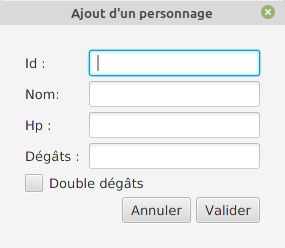
\includegraphics[width=0.35\textwidth, keepaspectratio]{img/personnageDialog.png}
		\end{figure}

	\section{Les items}

		Des items de toutes sorte peuvent être ajoutés : des items modifiant la santé, des armes, des défenses, différents types d'argent ainsi d'autre items basique (par exemple, une clé).

		Les items de santé, défenses et armes possède tous un champ "usure du matériel". il permet d'indiquer le nombre d'utilisation avant de voir l'item disparaître. Si l'item ne doit jamais disparaître on peut alors y mettre la valeur -1.

		Ces items peuvent ensuite être renseigné dans les noeuds qui en auront besoin, que ce soit pour les acheter ou pour les mettre à disposition du joueur. On peut également spécifier la nécessité de posséder un item pour pouvoir entreprendre un certains choix (cf : \nameref{sec:prerequis} page \pageref{sec:prerequis}).

		\begin{figure}[H]
			\centering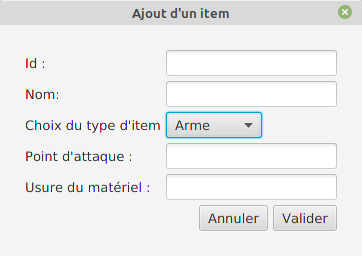
\includegraphics[width=0.35\textwidth, keepaspectratio]{img/itemDialog.png}
		\end{figure}

	\section{Les compétences}
		\label{sec:skills}

		Les compétences permettent de donner des pouvoir et des capacités à notre héro lui permettant d'accéder à différents choix. On peut par exemple imaginer des compétences lui permettant de pouvoir voler, être habille de ses mains ou posséder un sixième sens. Ils sont donc, pour le moment, un élément très simple qui possède qu'un ID ainsi qu'un nom.

		\begin{figure}[H]
			\centering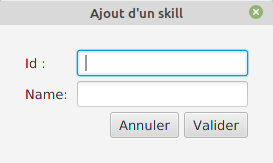
\includegraphics[width=0.35\textwidth, keepaspectratio]{img/skillDialog.png}
		\end{figure}

		Lors d'une prochaine mise à jour, il sera possible de créer des compétences avec différents effets (soins, dégats, ...). Les compétences peuvent uniquement être apprise dès le début du livre lors de la phase de "conception du personnage" (cf :  \nameref{subsubsec:persoCreationSkill} page \pageref{subsubsec:persoCreationSkill}).
